%!TEX root=./main.tex

%\section{Phase 1: Semi-automatic Registration of a Preoperative MRI to multiple Intraoperative Reference Images}
%% \subsection{The Initial Registration Stage}
%\label{sec:initialRegistration}
\subsection{Solving the Initial Registration}
\label{sec:registrationOverview}

\subsubsection{Solution Overview}
\fig{fig:initialRegOverview} shows the initial registration problem, which is challenging to solve for two main issues: \textit{(i)} the model to be registered is textureless and \textit{(ii)} the registration is non-rigid.
% We illustrate the problem in \fig{fig:initialRegOverview}. This stage is more challenging to solve than the tracking stage because \textit{(i)} we have no texture information associated with the organ's surface and \textit{(ii)} it is a deformable registration. 
To overcome these problems, our approach includes a dense 3D reconstruction of the organ's surface using an \emph{exploratory video} and SfM/MVS reconstruction, for which mature and open-source methods exist~\cite{Meshroom}. Given this reconstruction, we solve the initial registration with numerical optimization of a system that combines data constraints (organ-to-reconstruction distances and contour fragment distances) with constraints from the model's internal energy.

\subsubsection{Interventional 3D Reconstruction}
\label{sec:sfm}
%To perform the 3D reconstruction, sample images of the organ from different viewpoints and distances are required, known as \emph{keyframes}. We gather these as the surgeon performs an initial exploration of the organ (referred to as the \emph{exploratory phase}), 
During the exploratory video, the uterus is rotated by the surgeon's assistant using the cannula (\fig{fig:cannula}). It moves independently of background structures, so the scene cannot be reconstructed using SLAM, which requires the scene to be globally rigid. 
%Short version
% \SG{We developed a tool to automatically capture sharp keyframes with significant spatial displacement, as this improves the MVS reconstruction quality. We track SIFT features in the live feed using~\cite{Bouguet2001} and, based on the magnitude of their average 2D displacement, the UI hints when a new keyframe can be captured inviting to hold the camera still. On average we capture $N=15$ keyframes.}
%Extended version
\SG{We developed a new tool to capture sharp keyframes with significant mutual spatial displacement.
We extract SIFT keypoints from a frame and track them along the frames of the live feed~\cite{Bouguet2001}.
When the average 2D keypoint displacement exceeds a threshold (default, $\SI{100}{pixels}$) or too many keypoints are lost \wrt the initial frame (default, \SI{35}{\percent}), we consider that the camera has sufficiently moved. We are then ready to acquire a new keyframe and the UI  asks the surgeon to hold the camera still.
We then extract and track new keypoints and the keyframe is acquired when the maximum displacement remains below a threshold (default, $\SI{3}{pixels}$) for the last $M=15$ frames.
Then the process starts again until at least $N=15$ keyframes are acquired.}
% We then extract $N$ keyframes $\{K_1,\dots K_N\}$ (see \fig{fig:cannula}) with a default of $N=10$. We index these with $i\in [1,N]$. This is done by uniformly sampling the video into $N$ intervals. %  with a default $N=12$. 
% We sample the video into $N$ intervals (in practice, $N=10$) and we extract $N$ keyframes $\{K_1,\dots K_N\}$ (see \fig{fig:cannula}), one for each $i\in [1,N]$. 
% In order to select sharp images, which greatly improves the MVS reconstruction quality, each keyframe $K_i$ is select to be the one with the lowest visual motion. In order to assess the quantity of motion between consecutive frame pairs we compute the Sum-of-Absolute Difference (SAD) as measure of similarity.
% We sample the video into $N$ intervals (in practice, $N=10$) and we extract $N$ keyframes $\{K_1,\dots K_N\}$ (see \fig{fig:cannula}). 
% For each interval $i\in [1,N]$ we take the keyframe $K_i$ to be the one with the lowest visual motion, using the Sum-of-Absolute Difference (SAD) as the metric computed between consecutive frame pairs. This is done to improve the quality of the reconstruction because MVS works best with sharper images.
We use a touch-screen interface to manually segment the uterus roughly in the keyframes, so that the background is masked and only the organ is reconstructed. This takes a few seconds per keyframe.
% We then run a state-of-the-art dense SfM\&MVS open source library~\cite{AliceVision}. This provides a dense 3D point cloud $\mathcal{Q}\overset{\mathrm{def}}{=}\{\vet{q}_{1},\dots,\vet{q}_{M}\}$, $\vet{q}_{j}\in\mathbb{R}^{3}$, and the keyframe camera pose matrices $\mat{M}_i \in \mathcal{SE}_4$.
% These hold the laparoscope's rotation matrix $\mat{R}_{i}\in\mathcal{SO}_3$ and translation vector $\vet{t}_{i}\in\mathbb{R}^3$ relative to the point cloud. Recall that an MVS reconstruction is computed up to an unknown global scale factor $s$. We solve for $s$ jointly with registration.
We then run a state-of-the-art SfM/MVS open source library~\cite{AliceVision}. 
As output we obtain a dense 3D point cloud $\mathcal{Q}\overset{\mathrm{def}}{=}\{\vet{q}_{j}\}$, $\vet{q}_{j}\in\mathbb{R}^{3}$, and, for each keyframe, the relevant camera pose matrix $\mat{M}_i \in \mathcal{SE}_4$, holding the rotation matrix $\mat{R}_{i}\in\mathcal{SO}_3$ and translation vector $\vet{t}_{i}\in\mathbb{R}^3$ \wrt the point cloud.
We recall that all MVS reconstructions are  only computed up to an unknown global scale factor $s$. We solve for $s$ jointly with registration in \S\ref{sec:enOpt}.



%Recall that $\mathcal{Q}$ and $\vet{t}_i$ are defined up to the unknown scale factor $s\in\mathbb{R}^+$.
% We chose Photoscan because it has been shown to work well on laparoscopic data~\cite{Collins2013} and can produce far denser reconstructions than purely feature-based methods.

%There may exist some keyframes whose pose is not computable due to, \eg, insufficient visual overlap.
%We currently deal with this by simply removing the keyframe.
%Moreover, the point cloud $\mathcal{Q}$ may contain background and/or foreground structures that partially occlude the organ.
%In this case the human operator can crop them using a fast lasso-based user interface.
%To reduce time we do not require the cropping to be perfect.
%We allow some non-organ points to remain in $\mathcal{Q}$ and we deal with them by making the associated data term robust (see below).
 %There exist a large number of SfM packages one can use such as~\cite{visualSfM3DV,visualSfM3DVWebPage,photoscan}. We currently use Agisoft's Photoscan~\cite{photoscan} because it has been shown to work well on laparoscopic data~\cite{Collins2013} and can produce far denser reconstructions than purely feature-based methods. 
%In some instances SfM may fail, which typically occurs when the keyframe overlap is insufficient.
%This can usually be resolved by extracting more keyframes by doubling the number of intervals and re-running SfM.
%In the rare events in which SfM still fails, \eg, due to very weak texture, we find that image enhancement such as Storz's CLARA can help.
% Alternatively, SLAM could be tried because unlike SfM it exploits temporal continuity.

%Differently than~\cite{Collins2044} which used Photoscan~\cite{photoscan} as MVS tool, we used Meshroom~\cite{Meshroom}, which is an open-source 3D reconstruction software based on the photogrammetric library AliceVision~\cite{AliceVision}. 
%This can be easily integrated in our pipeline and it offers the advantage of easily customizing the settings and the reconstruction parameters to produce high quality 3D models.

\begin{figure}[t]
  \centering
  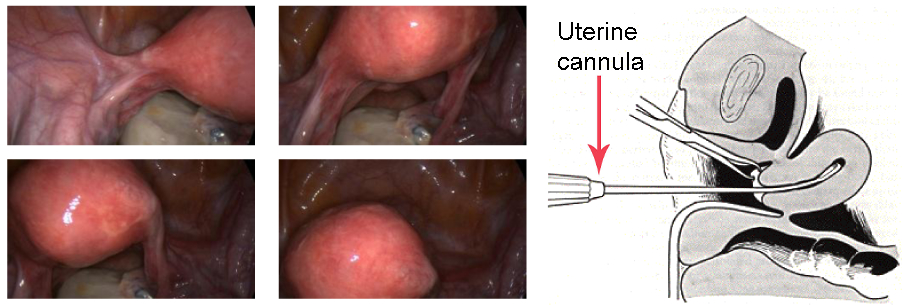
\includegraphics[width=0.79\columnwidth]{./figs/exploratory.pdf}
  \caption{Example keyframes from an exploratory video of a uterus undergoing cannula motion.}
	\label{fig:cannula}
\end{figure}


%In our experiments typically no more than $10$ images are required to obtain a good quality reconstruction.

%\begin{figure}[h]
%	\centering
%	\includegraphics[width=1.0\textwidth]{./figs/segmentationAndModel.pdf}
%	\caption{CAPTION}
%	\label{fig:deformableModel}
%\end{figure}

%\begin{figure}[h]
%	\centering
%	\includegraphics[width=1.0\textwidth]{./figs/optimisationTable.pdf}
%	\caption{CAPTION}
%	\label{fig:sfmExample}
%\end{figure}

%We summarise the initial registration process as follows. This is similar to~\cite{Collins2044} but with some important improvements that we list at the end of the paragraph. First a rough initialisation is made using a rigid transform and a small amount of manual assistance. 

\subsubsection{Silhouette Contours}
An occluding contour is a boundary in a 2D image between an object surface and another surface that is further away, that it partially occludes. This includes  \emph{self-occluding contours}, which are formed where the object self-occludes, and \emph{silhouette contours}, which are formed by the object and a background structure. Most organs are approximately convex, so self-occluding contours are rare events. \SG{By} contrast, silhouette contours are common, and we propose to use these to constrain the organ's shape during registration. We require the silhouette contours to be provided in a keyframe image (\fig{fig:initialRegOverview}). This is very difficult to automate because not all of the organ's boundaries in an image correspond to silhouette contours. Indeed, they are either silhouette contours, or contours formed by the silhouette of another structure occluding the organ. We illustrate this in \fig{fig:initialRegOverview} (top row) where abdominal fat occludes the posterior region of the uterus. The boundary between fat and the uterus conveys no information about the shape of the uterus.  
%we must both recover the organ's boundaries in an image, and infer which of those are silhouette contours compared with contours formed by another structure occluding the organ. 

%Consequently, extracting an organ's silhouette contours cannot be solved directly by organ segmentation, because this does not distinguish the above contour types. Furthermore, organ segmentation is itself a hard problem with laparoscopic images.
We therefore propose to extract silhouette contours with a fast semi-automatic process and a touch-screen interface. \SG{The keyframes are displayed} and the operator traces the organ's silhouette contours with a finger stroke. We apply the method of~\cite{Mortensen95intelligentscissors} to snap the finger stroke to the nearest image contour, based on active contours attracted to the dominant image edge adjacent. This is very fast and a keyframe is processed in a matter of seconds. %Occasionally, snapping may fail mainly in cases where the contour fragment is very low contrast. In these cases the operator sets the contour to inactive, meaning that it is not used during registration.



%We define a \emph{contour fragment} as a connected path in a keyframe image that corresponds with the organ's occluding contour. Recall that 

%%%%%%%%%%%%
%We formulate the problem as a non-linear energy-minimisation problem, with energies coming from prior and data terms.
%The prior term encodes the model's internal energy, which is used to regularise the problem.
%The data terms are illustrated in \fig{fig:initialRegOverview}.
%The first involves the point cloud reconstruction, and encourages the organ's surface mesh to fit to the point cloud.
%Importantly, this is a \emph{robust} data term, which accounts for the fact that the reconstruction may contain outliers or some residual background and/or occluding structures.
%The second data term complements the first and uses contour cues.
%Specifically, it is a silhouette contour term which makes the organ model's silhouette align to its associated contours in the keyframe images.
%This is complementary to the point cloud data term for two reasons.
%Firstly, we never usually reconstruct points reliably at these regions due to occlusions.
%Secondly, it anchors the organ's silhouette to the contour fragments, which is a strong constraint.
%We implement this data term with some manual assistance: a human operator marks in a keyframe where they can confidently see the organ's silhouette contours (\fig{fig:initialRegOverview}, first row).
%We call these \emph{contour fragments}.
%The operator does not need to mark contour fragments in all keyframes (it can be done with only one).
%If more keyframes are marked then we have more constraints marking contour fragments.
%Differently than our previous work~\cite{Collins2044}, the user can now mark these contours by means of a touch-screen interface using rough finger strokes.
%These strokes then guide an automatic refinement method based on intelligent scissors~\cite{Mortensen95intelligentscissors}.
%This reduces manual effort and speed up the process, which now typically takes, overall, less than $\SI{10}{\second}$ for a single keyframe.
%In general, $4$ to $6$ keyframes are enough.
%They also do not need to be contiguous. \todo{necessary to say?}
%Optionally, an anatomical landmark data term can also be included, which is used to align distinct landmarks that can be found on the organ's surface in the pre-operative and laparoscopic images.
%In the case of the uterus these can be the Fallopian tube/uterus junctions, which were manually located.
%Landmarks help guide the registration if the initialisation is poor or there is very strong deformation.
%In the presented experiments we do not use them in the optimisation process, so they are omitted from the energy function. 
%%%%%%%%%%%%%%%%%%%%%%%%


% The main improvements over~\cite{Collins2044} are summarised as follows:

%\paragraph{Overview.}
%We solve the initial registration in a similar way as described in~\cite{Collins2044} but with several key improvements. This is based on an energy-minimisation process where the energy encodes optical registration constraints from the keyframes and deformation priors from the organ's physical material. The energy is robust to handle common errors when pre-processing the keyframe images (\eg imperfect segmentation), and is minimised with iterative numerical optimisation. This requires an initial solution which can be computed depending on the context. We give details for how the initial solution is computed for the user study at the end of this section. An important assumption for solving the initial registration is that the organ does not deform during the exploratory phase. This allows us to reconstruct the interventional environment \emph{in 3D} with rigid Structure-from-Motion (SfM). With live organs slight deformation may be unavoidable, however if the deformations are small compared to the camera's motion then we can usually reconstruct the laparoscopic environment with a state-of-the-art dense SfM algorithm. The benefit of reconstructing the environment is twofold. Firstly, it allows us to calibrate the keyframe images, and this enables us to use \emph{all} keyframe images to constrain the initial registration problem. The second benefit is that the reconstruction gives information for the interventional 3D shape of the organ, which can be used to constrain the registration problem.

%\paragraph{Summary of improvements to~\cite{Collins2044} for solving the initial registration.} The main improvements are as follows:

% \begin{enumerate}[-,topsep=1pt]
% 	\item In~\cite{Collins2044} the deformable model used was a 3D affine model. 
%   This was shown to be sufficient for simple deformations of the human uterus but is not sufficient in general.
% We extend the approach to work with general biomechanical models.
% This requires changing the core energy function to include the model's internal energy (without this the problem is highly under-constrained), and to correct the interventional reconstruction's scale factor $s$.
% Note that in~\cite{Collins2044}, $s$ could be absorbed into the affine model's coefficients.
% This is generally not possible with biomechanical models because a change of scale affects the internal energy.
	
% 	\item In~\cite{Collins2044} the organ's surface was assumed to have disc topology.
% We  generalise this to arbitrary fixed topologies.
% 	\item We have sped up the process of marking contour fragments considerably with a touch-screen interface, where the operator marks them with rough finger strokes.
% These strokes then guide an automatic refinement method based on intelligent scissors~\cite{Mortensen95intelligentscissors}.
% This reduces manual effort, typically taking less than $\SI{10}{\second}$ for a single keyframe.
% \end{enumerate}  






 %Example keyframes and a dense SfM reconstruction for one of the user study kidneys is shown in Figure %\begin{figure}[h]
%	\centering
%	\includegraphics[width=1.0\textwidth]{./figs/sfm2.pdf}
%	\caption{CAPTION}
%	\label{fig:exampleKeyframesAndSfM}
%\end{figure}


%\paragraph{Contour fragments.} A human operator then traces contour fragments in one or more keyframes (we use a default of 4 uniformly sampled in time) using the touch-screen interface and intelligent scissoring, as described in point 3 above. This is a very fast process, however occasionally errors can happen when the fragment does not correctly snap to the right image position. This mostly occurs if the edge contrast is low. This could be dealt with by having the operator manually re-trace it without intelligent scissoring, but it would cost time. Instead we say that some errors in the contour fragments are unavoidable, and we deal with them by making the associated data term \emph{robust} to such errors, as described below. 

\subsection{Initialization}
\label{sec:Initialization}
Initially, \xref is initialized with a rigid transform $\mat{M}_a\in \mathcal{SE}_4$.
If the laparoscope is in a canonical position \wrt the organ, $\mat{M}_a$ can be considered known \emph{a priori}.
Otherwise, we devised an interactive and relatively simple procedure to provide a rough estimate of $\mat{M}_a$.
The method is based on solving PnP~\cite{Lepetit2009Epnp} between 3D points on the organ's surface model and their corresponding 2D points on one of the keyframes, selected interactively.
The operator can first freely rotate the 3D model to present it from a similar viewpoint as the keyframe.
\SG{Then they select at least $5$ 3D points on the 3D model and their corresponding points on the image.
We found that a good strategy is to select the $4$ equidistant points on the image along (but not on) the occluding contour and one roughly in the middle.
The corresponding points on the 3D model can be guessed following the same pattern.
Associating points from an untextured 3D model to its image is not in general a trivial task but we found that surgeons can easily perform the operation thanks to their detailed understanding of the anatomy.
The correspondences are not required to be accurate, as this only serves as rough initialization of the camera pose.}
%The estimated camera pose is used to initialize  $\mat{M}_a$.

% We initialize \xref with a rigid transform, denoted by $\mat{M}\in \mathcal{SE}_4$.
% In some cases $\mat{M}$ can be considered known \emph{a priori}, \eg if the laparoscope is assumed to be in a canonical position with respect to the organ.
% When this cannot be assumed, we compute it with a small amount of manual interaction as follows.
% A small number of point correspondences (at least four) are selected on the organ's surface model and one of the keyframe images.
% Without loss of generality, let this be the first keyframe $K_1$.
% We then compute a rigid transform  $\mat{M}_a$ from model coordinates to laparoscope coordinates, by fitting the correspondences using a PnP method~\cite{Lepetit2009Epnp}.
% The point correspondences are computed using an interactive user interface, where the model can be freely rotated to present it from a similar viewpoint as the keyframe's viewpoint. This significantly eases the operator's task. 

To provide an initialization of the reconstruction scale factor $s$, we apply $\mat{M}_a$ to the model.
We then use OpenGL to render a synthetic image of it using the calibrated intrinsic parameters of the laparoscope. 
OpenGL's $z$-buffer provides a depth map $d(x,y)$ from which we can compute $s$ by comparing depths in $d$ to depths in $\mathcal{Q}$.
% We initialize the reconstruction scale factor $s$ as follows. First we transform the model by $\mat{M}_a$ and render it using the OpenGL rendering engine, using the same intrinsic parameters as the laparoscope, thus obtaining a depth map $d(x,y)$ from OpenGL's $z$-buffer. We then compute $s$ by comparing depths in $d$ to the depths of $\mathcal{Q}$. 
Specifically, for a 3D point $\vet{q}_j$, an estimate of $s$ is  $s_j=d(x_j,y_j)/\tilde{d}_j$, where $\tilde{d}_j$ is the depth of $\vet{q}_j$, and $(x_j,y_j)$ its corresponding 2D point.
The robust estimate is given by the median over all points, $s=\mathrm{median} \{s_j\}$. 

% Specifically, let $\tilde{d}_j$ be the depth of $\vet{q}_j$ in keyframe $K_1$, and $(x_j,y_j)$ be its 2D position in the keyframe's image. We can then estimate $s$ by $s\approx d(x_j,y_j)/\tilde{d}_j$. To compute $s$ robustly, we use the median estimate using all points. Finally, the transform $\mat{M}$ is given by the composition $\mat{M} = \mat{M}_s\,\mat{M}^{-1}_i\,\mat{M}^{-1}_s\,\mat{M}_a$, where $\mat{M}_s$ is an isotropic scaling by $s$. 

\subsection{Energy-based Optimization}
\label{sec:enOpt}
We describe the registration energy function and optimization process. To improve clarity we assume all image points in normalized camera coordinates, which is obtained from the intrinsic calibration, and thus define camera projection as
$\pi(\left[x,y,z\right]^{\top})\overset{\mathrm{def}}{=}\left[x,y\right]^{\top}/z$. 
Besides the model's internal energy $\Einternal(\vet{x})$, the energy function $E(\vet{x},s)\in\mathbb{R}^+$ consists of two other terms.
We introduce a point cloud data term \Epoint to help the organ's surface fit the reconstructed point cloud.
To constrain the organ's silhouette contours to fit the silhouette contour fragments we also include a contour data term \Econtour. 
Thus, the energy $E(\vet{x},s)$ is defined as:
\begin{equation}
\label{eq:totalCost}
\begin{split}
E(\vet{x},s)=\Epoint(\vet{x},s;\mathcal{Q}) & + \lambdaContour\Econtour(\vet{x},s)
% \\;\mathcal{C}_{1},\dots ,\mathcal{C}_{N}
% & 
+\lambdaInternal\Einternal(\vet{x}),
\end{split}
\end{equation}
\noindent where $\lambdaContour$ and $\lambdaInternal$ are scalar weights (\SG{with defaults} $\lambdaContour=100$ and $\lambdaInternal=50$).

% The energy function $E(\vet{x},s)\in\mathbb{R}^+$ consists of the point cloud data term \Epoint, which encourages the organ's surface to fit to the reconstructed point cloud $\mathcal{Q}$, the contour data term \Econtour, which encourages the organ's silhouette contours to fit to the silhouette contour fragments, and the model's internal energy $\Einternal(\vet{x})$:
% \begin{equation}
% \label{eq:totalCost}
% \begin{split}
% E(\vet{x},s)=\Epoint(\vet{x},s;\mathcal{Q}) & + \lambdaContour\Econtour(\vet{x},s;\mathcal{C}_{1},\dots ,\mathcal{C}_{N})\\
% & +\lambdaInternal\Einternal(\vet{x}),
% \end{split}
% \end{equation}
% \noindent where $\lambdaContour$ and $\lambdaInternal$ are scalar weights (typically, $\lambdaContour=100$ and $\lambdaInternal=50$).
% The set $\mathcal{C}_i$ denotes all pixels on the contour fragments in keyframe $i$. 

For the point cloud data term \Epoint we use an ICP-based energy term: it uses a set of \emph{virtual point correspondences} $\mathcal{P}=\{\vet{p}_j\}$ with $|\mathcal{Q}|=|\mathcal{P}|$, where $\vet{p}_j\in\partial \Omega$ is the unknown position of point $\vet{q}_{j}$ on the organ's surface mesh $\Omega$.
For a given $(\vet{x},s)$, \Epoint is computed by first transforming $\Omega$ according to $\ensuremath{f(\cdot;\vet{x})}$ and applying the estimated scale factor $s$ to the point cloud, so that $\hat{\vet{q}}_{j}\gets s\,\vet{q}_{j}$.
Then, $\vet{p}_j$ is set to the closest point to $\hat{\vet{q}}_{j}$ on the surface's mesh.
Similarly to the point-to-plane distance function of ICP with rigid objects, \Epoint uses a robust point-to-plane distance function that allows the model to slide over the point cloud without resistance:
\begin{equation}
\Epoint(\vet{x},s;\mathcal{Q})=\frac{1}{M}\sum_{j=1}^{M}\rho\left(\dplane\left(v_{j}(\vet{x}),\hat{\vet{q}}_{j}\right)\right),
\end{equation}
where $v_{j}(\vet{x})\in\mathbb{R}^4$ gives the organ surface's tangent plane at $f(\vet{p}_{j})$.
The function $\dplane(\vet{v},\vet{q})$ gives the signed distance between a plane $\vet{v}$ and a 3D point $\vet{q}$.
The function $\rho:\mathbb{R}\rightarrow\mathbb{R}^{+}$ is an \emph{M-estimator}. % and it is designed to robustly align the reconstructed point $\hat{\vet{q}}_{j}$ with the organ's surface. 
The MVS reconstruction may contain points off the organ or poorly reconstructed; these are discarded by the M-estimator.
We experimented with different types of estimators and found that a pseudo-L1 $\rho({x})\overset{\mathrm{def}}{=}\sqrt{{x}^{2}+\epsilon}$ offers good results (\SG{with default} $\epsilon = 10^{-4}$).

% We construct \Epoint using an ICP-based energy term.
% This works using a set of \emph{virtual point correspondences} $\mathcal{P}=\{\vet{p}_1,\dots \vet{p}_M\}$ with $\vet{p}_j\in\partial \Omega$ denoting the unknown position of point $j$ on the organ's surface mesh. 
% For a given $(\vet{x},s)$ we compute \Epoint as follows. First we transform the organ's surface mesh according to $\ensuremath{f(\cdot;\vet{x})}$ and rescale the point cloud with $\hat{\vet{q}}_{j}\gets s\,\vet{q}_{j}$.
% We then set $\vet{p}_j$ as the closest point to $\hat{\vet{q}}_{j}$ on the surface's mesh.
% We define \Epoint using a robust point-to-plane distance function, which is inspired by point-to-plane ICP with rigid objects.
% This allows the model to slide over the point cloud without resistance, and is defined as follows:
% \begin{equation}
% \Epoint(\vet{x},s;\mathcal{Q})=\frac{1}{M}\sum_{j=1}^{M}\rho\left(\dplane\left(v_{j}(\vet{x}),\hat{\vet{q}}_{j}\right)\right).
% \end{equation}
% \noindent The function $v_{j}(\vet{x})\in\mathbb{R}^4$ gives the organ surface's tangent plane at $f(\vet{p}_{j})$.
% The function $\dplane(\vet{v},\vet{q})$ gives the signed distance between a plane $\vet{v}$ and a 3D point $\vet{q}$.
% The function $\rho:\mathbb{R}\rightarrow\mathbb{R}^{+}$ is an \emph{M-estimator} and is crucial to achieve robust registration.
% Its purpose is to align the reconstructed point $\hat{\vet{q}}_{j}$ with the organ's surface, but to do so robustly to account for non-organ points being in $\mathcal{Q}$ or poorly reconstructed points.
% The model should not align these points, and the M-estimator facilitates this by reducing their influence on the energy.
% We have tested various types and good results are obtained with pseudo-L1 $\rho({x})\overset{\mathrm{def}}{=}\sqrt{{x}^{2}+\epsilon}$ with $\epsilon = 10^{-4}$.

Similarly, \Econtour uses virtual point correspondences on the organ surface mesh's occluding contours.
More explicitly, for a given estimate $(\vet{x},s)$ and a given keyframe $i$, we generate a set of virtual correspondences $\mathcal{R}_i=\{\vet{r}_1,\dots ,\vet{r}_{C(i)}\}$
containing, for each contour pixel $\vet{c}_k$, the unknown position $\vet{r}_k\in\partial \Omega$  of its corresponding 3D point on the model's surface.
To compute the correspondence we first apply $\ensuremath{f(\cdot;\vet{x})}$ to the organ's surface mesh, and we bring the model in the reference frame of the camera $i$ using $(\mat{R}_{i}, s\,\vet{t}_{i})$.
Then
% , using the same intrinsic parameters as the laparoscope, 
we render the surface mesh as described in \sect{sec:Initialization} and store all the pixels on the silhouette boundary in a set $\mathcal{B}$. 
Let $\mathcal{C}_i$  the set of all pixels belonging to the contour fragments in keyframe $i$.
We compute for each contour pixel $\vet{c}_k\in \mathcal{C}_j$ its closest point $\vet{b}_k\in \mathcal{B}$.
Finally, we set $\vet{r}_k$ as the 3D position of $\vet{b}_k$, computed using the render's depth buffer.
From all the correspondences $\mathcal{R}_i$, \Econtour is computed as:
\begin{equation}
\label{eq:contour}
\begin{split}
% ;\mathcal{C}_{1},\dots,\mathcal{C}_{N}
 & \Econtour(\vet{x},s) = \frac{1}{C}\sum_{i=1}^{N}\sum_{\substack{\vet{c}_{k}\in\mathcal{C}_{i}\\\vet{r}_{k}\in\mathcal{R}_{i}}}\rho\left(\|\pi\left(f(\vet{r}_{k})\right)-\vet{c}_{k}\|\right),
\end{split}
\end{equation}
\noindent where $C$ is the total number of contour fragment pixels.
Similarly to \Epoint, we use the M-estimator $\rho$ for robustness.

% We construct \Econtour similarly with virtual point correspondences.
% Specifically, for a given pair $(\vet{x},s)$ and a given keyframe $i$ we construct a set of virtual correspondences $\mathcal{R}_i=\{\vet{r}_1,\dots ,\vet{r}_{C(i)}\}$ where $\vet{r}_k\in\partial \Omega$ denotes the unknown position of the $k^{th}$ contour fragment pixel $\vet{c}_k$ on the model's surface.
% The virtual correspondences are points on the organ surface mesh's occluding contours, and are computed as follows.
% First we transform the organ's surface mesh according to $\ensuremath{f(\cdot;\vet{x})}$, then transform it to laparoscope coordinates using $(\mat{R}_{i}, s\,\vet{t}_{i})$.
% We render the surface mesh, using the same intrinsic parameters as the laparoscope.
% We then take the render's silhouette and store all the pixels on the render's boundary in a set $\mathcal{B}$.
% For each contour fragment pixel $\vet{c}_k\in \mathcal{C}_j$ we compute its closest point $\vet{b}_k\in \mathcal{B}$  and form a correspondence with it.
% We then compute the 3D position of $\vet{b}_k$ using the render's depth buffer, and assign this position to $\vet{r}_k$.
% We then evaluate \Econtour as the alignment error from all correspondences:
% \begin{equation}
% \label{eq:contour}
% \begin{split}
%  & \Econtour(\vet{x},s;\mathcal{C}_{1},\dots,\mathcal{C}_{N}) = \\ 
%  &  \frac{1}{C}\sum_{i=1}^{N}\sum_{\substack{\vet{c}_{k}\in\mathcal{C}_{i}\\\vet{r}_{k}\in\mathcal{R}_{i}}}\rho\left(\|\pi\left(f(\vet{r}_{k})\right)-\vet{c}_{k}\|_{2}\right),
% \end{split}
% \end{equation}
% \noindent where $C$ is the total number of contour fragment pixels.
% Here the M-estimator $\rho$ is also used to handle the fact that some contour fragments may be erroneous, which can occurs if the contour fragment incorrectly snaps at low-contrast edges. 

% and we give details for each test case in the experimental section. The weights $\lambdaContour$ and $\lambdaInternal$ are fixed in all experiments at $\lambdaContour=100$ and $\lambdaInternal=50$. 

\subsection{Optimisation}
In order to improve convergence, we use a stiff-to-flexible strategy to optimize $E$. We start with a stiff model, we optimize $E$, and then we reduce the stiffness to account for more deformation.
We usually use $6$ stiffness levels, in which the value of $\lambdaInternal$ is halved \wrt the previous level, \ie $\lambdaInternal(l)=\lambdaInternal(l-1)/2$.
At each level we alternate between computing the virtual correspondence sets ($\mathcal{R}_i$ and $\mathcal{P}$) and optimising $E$, via Gauss-Newton iterations with backtracking line search until either convergence or a maximum of $20$ iterations is reached.
% We optimize $E$ using a stiff-to-flexible strategy. This is to improve convergence by starting with a stiff model, optimising $E$, then reducing the stiffness to account for more and more deformation. We use a default of $l=6$ stiffness levels with $\lambdaInternal(l)=2\,\lambdaInternal(l-1)$. For each level we alternate between computing the virtual correspondence sets ($\mathcal{R}_i$ and $\mathcal{P}$) and optimising $E$, via a Gauss-Newton iteration with backtracking line search. This continues until either convergence is reached or $20$ iterations have passed. %At the final stiffness level we optimize until convergence. 
%Convergence however is not guaranteed because of the point-to-plane distance function in \Epoint. Specifically, the energy may increase after $\mathcal{P}$ is re-computed. We handle this by using the point-to-point distance at the final level, because this ensures $E$ will decrease at each iteration, and optimize until convergence.
